%%%%%%%%%%%%%%%%%%%%%%%%%%%%%%%%%%%%%%%%%%%%%%%%%%%%%%%%%%%%%%%%%%%%%%%%%%%%
%% Trim Size: 9.75in x 6.5in
%% Text Area: 8in (include Runningheads) x 5in
%% ws-ijmpcs.tex   :   23-7-2010
%% Tex file to use with ws-ijmpcs.cls written in Latex2E.
%% The content, structure, format and layout of this style file is the
%% property of World Scientific Publishing Co. Pte. Ltd.
%% Copyright 1995, 2002 by World Scientific Publishing Co.
%% All rights are reserved.
%%%%%%%%%%%%%%%%%%%%%%%%%%%%%%%%%%%%%%%%%%%%%%%%%%%%%%%%%%%%%%%%%%%%%%%%%%%%
%%

%\documentclass[draft]{ws-ijmpcs}
\documentclass{ws-ijmpcs}

\begin{document}

\markboth{C. A. Graeff \& D. P. Menezes}
{NJL/eNJL phase diagram}

%%%%%%%%%%%%%%%%%%%%% Publisher's Area please ignore %%%%%%%%%%%%%%%
%
\catchline{}{}{}{}{}
%
%%%%%%%%%%%%%%%%%%%%%%%%%%%%%%%%%%%%%%%%%%%%%%%%%%%%%%%%%%%%%%%%%%%%

\title{The QCD phase-diagram obtained from the NJL and the extended-NJL models for quark and hadron phases}

\author{Clebson A. Graeff}

\address{Departamento de F\'isica, Universidade Tecnol\'ogica Federal do Paran\'a, Via do Conhecimento, Km 1 CEP 85503-390\\
Pato Branco, Paran\'a,
Brazil
cgraeff@utfpr.ed.br}

\author{D\'ebora P. Menezes}

\address{Departamento de F\'isica, Universidade Federal de Santa Catarina\\ Florian\'opolis, SC, CP 476, CEP 88.040-900, Brazil\\
debora.p.m@ufsc.br}

\maketitle

\begin{history}
\received{Day Month Year}
\revised{Day Month Year}
\published{Day Month Year}
\end{history}

\begin{abstract}
We analyse the hadron/quark phase transition described by the Nambu-Jona-Lasinio (NJL) model [quark phase] and the extended Nambu-Jona-Lasinio model (eNJL) [hadron phase]. While the original formulation of NJL model is not capable of describing hadronic properties due to its lack of confinement, it can be extended with a scalar-vector interaction so it exhibits this property, the so-called  eNJL model. As part of this analysis, we obtain the equations of state within the SU(2) versions of both models for the hadron and the quark phases and determine the binodal surface. 
\keywords{Phase-transition; NJL; binodal.}
\end{abstract}

\ccode{PACS numbers:}

%%%%%%%%%%%%%%%%%%%%%%%
\section{Motivation}

The study of the QCD phase-diagram is relevant to the understanding of many aspects of the physics in our universe. Two of the aspects of interest are related to relativistic heavy ion collisions (low densities, high temperatures) and stars (high densities, low temperatures). However, the direct solution of QCD is not possible at finite chemical potential.

Given the importance of the study of the phases and the phase separation boundaries, we propose an investigation of the hadron/quark phase transition within a two phase model.

%%%%%%%%%%%%%%%%%%%%%%%%%%%%%
\section{Quark phase matter}

The quark phase is described by a SU(2) NJL model lagrangian, including a vector-isoscalar term, given by \cite{Buballa2005}
\begin{equation}\label{Eq:LagNJL-SU2-Bub}
	\mathcal{L} =\bar{\psi}(i\gamma^\mu\partial_\mu - m_0)\psi + G_S[(\bar{\psi}\psi)^2 + (\bar{\psi}i\gamma_5\vec{\tau}\psi)^2] - G_V(\bar{\psi}\gamma^\mu \psi)^2.
\end{equation}
%
Here $\psi$ represents the quark field, $m_0$ the quark bare mass, and $G_S$ and $G_V$ are coupling constants that are chosen by fitting the pion mass $m_\pi = 135.0~\rm{MeV}$ and decay constant $f_\pi = 92.4~\rm{MeV}$. As the theory is non-renormalizable, a momentum cutoff $\Lambda$ is employed, which acts as a new parameter.

\begin{table}[ht]
\tbl{Parameters sets for the lagrangian density~\protect\eqref{Eq:LagNJL-SU2-Bub} \protect\cite{Buballa1996,Buballa2005}.}
{\begin{tabular}{@{}lcccccccc@{}}\toprule
Model &  $\Lambda$ & $G_S$ ($\rm{fm}^2$) & $G_V$ ($\rm{fm}^2$) & $m_0$ (MeV) & $m$ (MeV) \\ \colrule
$B_1$ & 650 & 0.19721 & -- & 0 & 313 \\
$B_2$ & 600 & 0.26498 & -- & 0 & 400 \\
$B_3$ & 570 & 0.34034 & -- & 0 & 500 \\
$B_2^R$ & 587.9 & 0.27449 & 0 & 5.6 & 400 \\
$B_2^R|_{G_V}$ & 587.9 & 0.27449 & $G_V \propto G_S$ & 5.6 & 400\\
\botrule
\end{tabular} \label{Tab:Parametros_NJL}}
\end{table}

%%%%%%%%%%%%%%%%%%%%%%%%%%%%%%
\section{Hadron phase matter}

Even though the original NJL model is unable to describe the saturation properties of the nuclear matter, this can be fixed by the inclusion of extra channels which combine the scalar and vector terms~\cite{Koch1987}. An extended NJL model (eNJL)~\cite{Pais2016} which includes such channel is given by the lagrangian density
\begin{equation}\label{Eq:Lagrangiana_eNLJ_Pais}
\begin{split}
	\mathcal{L} =&~ \bar{\psi}(i\gamma^\mu\partial_\mu - m_0)\psi + G_s[(\bar{\psi}\psi)^2 + (\bar{\psi}i\gamma_5\vec{\tau}\psi)^2] - G_v(\bar{\psi}\gamma^\mu\psi)^2 \\
	& - G_\rho[(\bar{\psi}\gamma^\mu\vec{\tau}\psi)^2 + (\bar{\psi}\gamma_5\gamma^\mu\vec{\tau}\psi)^2] - G_{sv}[(\bar{\psi}\psi)^2 + (\bar{\psi}i\gamma_5\vec{\tau}\psi)^2](\bar{\psi}\gamma^\mu\psi)^2 \\
	& - G_{v\rho}(\bar{\psi}\gamma^\mu\psi)^2[(\bar{\psi}\gamma^\mu\vec{\tau}\psi)^2 + (\bar{\psi}\gamma_5\gamma^\mu\vec{\tau}\psi)^2] \\
	& - G_{s\rho} [(\bar{\psi}\psi)^2 + (\bar{\psi}i\gamma_5\vec{\tau}\psi)^2][(\bar{\psi}\gamma^\mu\vec{\tau}\psi)^2 + (\bar{\psi}\gamma_5\gamma^\mu\vec{\tau}\psi)^2].
\end{split}
\end{equation}
%
where $\psi$ represents the nucleon field and the constants $G_i$ represents the coupling constants for the different channels.
%
\begin{table}[hb]
\tbl{Parameters sets for the lagrangian density~\protect\eqref{Eq:Lagrangiana_eNLJ_Pais} \protect\cite{Pais2016}.}
{\begin{tabular}{@{}lcccccccc@{}}\toprule
Model & $G_s$ ($\rm{fm}^2$) & $G_v$ ($\rm{fm}^2$) & $G_{sv}$ ($\rm{fm}^8$) & $G_\rho$ ($\rm{fm}^2$) & $G_{v\rho}$ ($\rm{fm}^8$) & $G_{s\rho}$ ($\rm{fm}^8$) & $\Lambda$ (MeV) & $m$ (MeV) \\ \colrule
eNJL1 & 4.855 & 4.65 & -6.583 & 0.5876 & 0 & 0 & 388.189 & 0 \\
eNJL1$^m$ & 1.3833 & 1.781 & -2.943 & 0.7 & 0 & 0 & 478.248 & 450 \\
eNJL1$_{\omega\rho 1}$ & 4.855 & 4.65 & -6.583 & 0.5976 & -1 & 0 & 388.189 & 0 \\
eNJL1$_{\omega\rho 2}$ & 4.855 & 4.65 & -6.583 & 0.6476 & -6 & 0 & 388.189 & 0 \\
eNJL2 & 3.8 & 3.8 & -4.228 & 0.6313 & 0 & 0 & 422.384 & 0 \\
eNJL2$^m$ & 1.078 & 1.955 & -2.74 & 0.75 & 0 & 0 & 502.466 & 450 \\
eNJL2$_{\omega\rho 1}$ & 3.8 & 3.8 & -4.228 & 0.6413 & -1 & 0 & 422.384 & 0 \\
eNJL3 & 1.93 & 3.0 & -1.8 & 0.65 & 0 & 0 & 534.815 & 0 \\
eNJL3$_{\sigma\rho 1}$ & 1.93 & 3.0 & -1.8 & 0.0269 & 0 & 0.5 & 534.815 & 0 \\
eNJL1$^m_{\sigma\rho 1}$ & 1.3833 & 1.781 & -2.943 & 0.0739 & 0 & 1 & 478.248 & 450 \\
eNJL2$^m_{\sigma\rho 1}$ & 1.078 & 1.955 & -2.74 & -0.1114 & 0 & 1 & 502.466 & 450 \\
\botrule
\end{tabular}\label{Tab:Parametros_eNJL}}
\end{table}


%%%%%%%%%%%%%%%%%%%
\section{Binodals}

The QCD phase-diagram is characterized by potentially multiple phases, whose phase separation boundaries are referred as \emph{binodals}. Over those boundaries, the phases from the regions of either side of the boundary can coexist. The binodals may be determined using the Gibbs' conditions \cite{Cavagnoli2011}:
\begin{align}
\mu_B^Q &= \mu_B^H & T^Q &= T^H & P^Q &= P^H
\end{align}
%
with
\begin{align*}
\mu_B^H &= \frac{\mu_p + \mu_n}{2} & 	\mu_B^Q &= \frac{3}{2} (\mu_u + \mu_d) = 3 \mu_q.
\end{align*}

\noindent{}where the indexes $H$ and $Q$ refer to the hadrons and quarks phases. The phase coexistence may then be obtained by simply plotting $P^i \times \mu_B^i$, $i = Q, H$, and looking for the intersection of both lines.

%%%%%%%%%%%%%%%%%%%%
\section{Results}

We determine the equations of state for both models at $T = 0$ and proton fraction $y_p = 0.5$. The realized phase of the system is the one which maximizes the pressure. This means that the crossing of the lines, as in Figure~\ref{Fig:Pressure_func_chemical_pot}, indicates a phase transition.
%
In Table~\ref{Tab:Transition_chemical_pot} we show the chemical potential $\mu_B^i$ at phase-transition for combinations of parameterizations of Tables~\ref{Tab:Parametros_NJL} and~\ref{Tab:Parametros_eNJL}. Combinations for which there is no transition are ommited.

\begin{figure}
\centering
\caption{The crossing point at a $P^i \times \mu_B^i$ plot indicate the phase-coexistence.\label{Fig:Pressure_func_chemical_pot}}
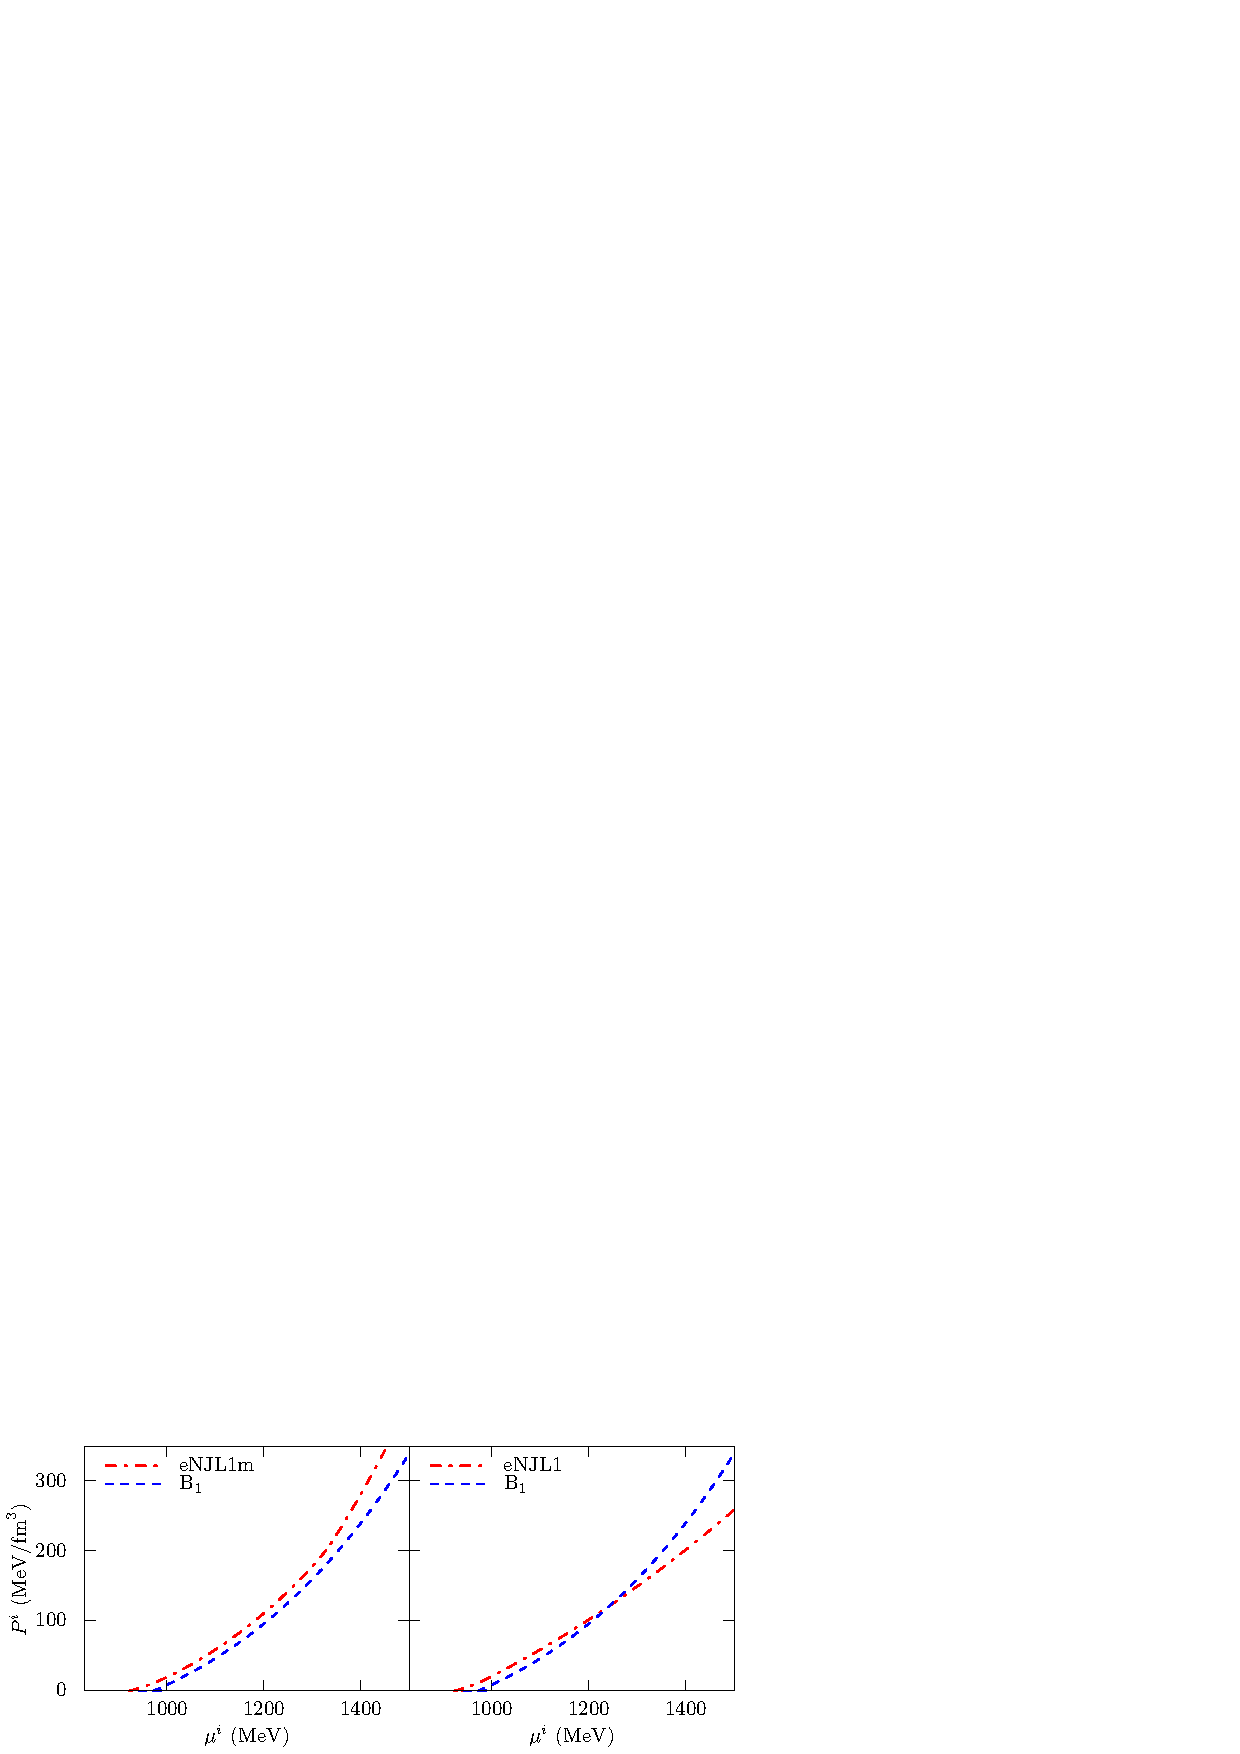
\includegraphics[width=10cm]{quark-hadron_phase_transition.pdf}
\end{figure}

\begin{table}[htb]
\tbl{Chemical potential $\mu_B^i$ at crossing point por different parameterization combinations..}
{\begin{tabular}{@{}ccccccccc@{}} \toprule
$Q$ & $H$ & $\mu_B^i$ (MeV) & $P^i$ ($\frac{\rm{MeV}}{\rm{fm}^3}$) && $Q$ & $H$ & $\mu_B^i$ (MeV) & $P^i$ ($\frac{\rm{MeV}}{\rm{fm}^3}$)  \\ \colrule
$B_1$ & eNJL1 & 1244 & 122                    &&   $B_2$ & eNJL3$_{\sigma\rho 1}$ & 1571 & 361    \\
$B_1$ & eNJL1$_{\omega\rho 1}$ & 1244 & 122   &&   $B_3$ & eNJL1 & 1615 & 330                 \\
$B_1$ & eNJL1$_{\omega\rho 2}$ & 1244 & 122   &&   $B_3$ & eNJL1$_{\omega\rho 1}$ & 1615 & 331    \\
$B_1$ & eNJL2 & 1373 & 216                    &&   $B_3$ & eNJL1$_{\omega\rho 2}$ & 1615 & 331    \\
$B_1$ & eNJL2$^m$ & 1279 & 145                   &&   $B_3$ & eNJL2 & 1700 & 456                 \\
$B_1$ & eNJL2$^m_{\sigma\rho 1}$ & 1279 & 145  &&   $B_3$ & eNJL2$_{\omega\rho 1}$ & 1700 & 456    \\
$B_1$ & eNJL2$_{\omega\rho 1}$ & 1373 & 216   &&   $B_3$ & eNJL3 & 1744 & 530                 \\
$B_1$ & eNJL3 & 1313 & 169                    &&   $B_3$ & eNJL3$_{\sigma\rho 1}$ & 1744 & 530    \\
$B_1$ & eNJL3$_{\sigma\rho 1}$ & 1313 & 169   &&   $B_2^R$ & eNJL1 & 1475 & 244                \\
$B_2$ & eNJL1 & 1460 & 235                    &&   $B_2^R$ & eNJL1$_{\omega\rho 1}$ & 1475 & 244   \\
$B_2$ & eNJL1$_{\omega\rho 1}$ & 1460 & 235   &&   $B_2^R$ & eNJL1$_{\omega\rho 2}$ & 1475 & 244   \\
$B_2$ & eNJL1$_{\omega\rho 2}$ & 1460 & 235   &&   $B_2^R$ & eNJL2 & 1570 & 354                \\
$B_2$ & eNJL2 & 1557 & 343                    &&   $B_2^R$ & eNJL2$^m$ & 1730 & 587               \\
$B_2$ & eNJL2$^m$ & 1675 & 506                   &&   $B_2^R$ & eNJL2$^m_{\sigma\rho 1}$ & 1730 & 587  \\
$B_2$ & eNJL2$^m_{\sigma\rho 1}$ & 1675 & 506  &&   $B_2^R$ & eNJL2$_{\omega\rho 1}$ & 1570 & 354   \\
$B_2$ & eNJL2$_{\omega\rho 1}$ & 1557 & 343   &&   $B_2^R$ & eNJL3 & 1587 & 376                \\
$B_2$ & eNJL3 & 1571 & 361                    &&   $B_2^R$ & eNJL3$_{\sigma\rho 1}$ & 1587 & 376   \\
\botrule
\end{tabular} \label{Tab:Transition_chemical_pot}}
\end{table}


%%%%%%%%%%%%%%%%%%%%%%%%%%%%%%%%%%%%%%
\section{Conclusions}

From the leftmost plot at Figure~\ref{Fig:Pressure_func_chemical_pot}, we can see that not all combinations of parameterizations produce a system in which a phase-transition is favored. Another manifestation of the dependence of the results in the choice of parameterizations is the range of chemical potential for which the transition takes place: it spans from 1248.3~MeV to 1744.3~MeV, a 40\% difference in relation to the lowest value. This indicates that the choice of parameterizations to produce a complete phase-diagram should made with care.

As a next step on this analysis, we shall turn our attention to expand our results for finite temperature and obtain the binodal sections.

%%%%%%%%%%%%%%%%%%%%
\section{References}
%%%%%%%%%%%%%%%%%%%%

\begin{thebibliography}{00}    %for 1 digit

%%journal paper
\bibitem{Pais2016} H. Pais, D. P. Menezes and C. Providência, {\it Phys. Rev. C} {\bf 93} (2016) 065805.

\bibitem{Buballa1996} M. Buballa, {\it Nuclear Physics A} {\bf 611} (1996) 393-408

\bibitem{Buballa2005} M. Buballa, {\it Phys. Rep.} {\bf 407} (2005) 205-376

\bibitem{Lee2013} T. Lee, Y. Tsue, J. da Provid{\^e}ncia, C. Provid{\^e}ncia, M. Yamamura, {\it Prog. Theor. Exp. Phys.} {\bf 2013} 013D02

\bibitem{Tsue2010} Y. Tsue, J. da Provid{\^e}ncia, C. Provid{\^e}ncia, M. Yamamura {\it Progress of Theoretical Physics} {\bf 123} (2010)

\bibitem{Menezes2003} D. P. Menezes, C. Providência, {\it Phys. Rev. C} {\bf 68} (2003) 035804

\bibitem{Koch1987} V. Kock, T. S. Biro, J. Kunz, U. Mosel, {\it Physics Letters B} {\bf 185} (1987) 1-5

\bibitem{Cavagnoli2011} R. Cavagnoli, C. Providência, D. P. Menezes, {\it Phys. Rev. C} {\bf 83} (2011) 045201

\end{thebibliography}

\end{document}

